\subsection{ORB: Oriented FAST and Rotated BRIEF}
\label{sec:ORB}
ORB basiert auf dem FAST-Algorithmus f�r die Schl�sselpunktsuche und dem BRIEF-Algorithmus f�r die Generierung von Deskriptoren

\paragraph{Sch�sselpunktsuche mit FAST}

Der FAST-Algorithmus sucht nach Eckpunkten in einem Bild. Dazu wird um jeden Pixel im Bild ein Kreis mit 16 Randpixeln gezogen. Der betrachtete Kandidat-Pixel ist genau dann ein Eckpunkt, wenn eine bestimmte Anzahl an aneinander grenzenden Randpixel heller oder dunkler sind als der Kandidat-Pixel plus oder minus einem bestimmten Schwellenwert. \cite[S. 4]{fast2006}

\begin{figure}[h]
\centering
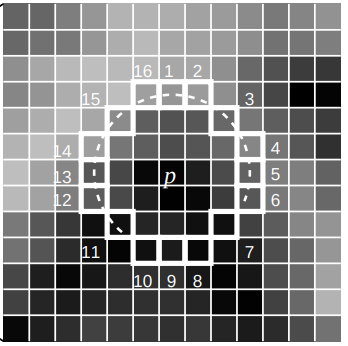
\includegraphics[scale=.7]{Abbildungen/fast}
\caption{Randpixel um Kandidat-Pixel aus \cite[S. 4]{fast2006}}
\label{fig:pixelkreis}
\end{figure}

Bei der Implementation in ORB m�ssen 9 der 16 Randpunkte heller oder dunkler als der Kandidat-Pixel sein, damit dieser sich als Randpunkt qualifiziert. 
Zudem wird die "Harris corner measure" genutzt um Randpunkte herauszufiltern. 
Dazu wird jedem Schl�sselpunkt ein Wert zugeteilt, der aussagt, wie wahrscheinlich es ist, dass es sich bei dem Schl�sselpunkt um einen Eckpunkt handelt. Der Schwellenwert, um sich als Eckpunkt zu qualifizieren, wird niedrig genug gesetzt um eine bestimmte Mindestanzahl an Schl�sselpunkten zu erreichen. 
Die Mindestanzahl an Schl�sselpunkten, kann dabei je nach Anwendungsfall variieren. Es muss gen�gend Schl�sselpunkte geben, um das Bild zu beschreiben. 
Gleichzeitig m�chte man aber Schl�sselpunkte vermeiden deren Deskriptoren nicht zuverl�ssig verglichen werden k�nnen. \cite[S. 2565]{orb2011}

Die durch FAST gefundenen Schl�sselpunkte sind anders als bei SIFT noch nicht Robust gegen�ber Rotations- und Aufl�sungsunterschieden. 
Um Invarianz gegen�ber Aufl�sungsunterschieden entgegenzuwirken, generiert ORB �hnlich wie SIFT (Abschnitt ~\ref{sec:Extrempunktsuche} mehrere niedriger aufgel�ste Varianten des Originalbilds. 
F�r jede Aufl�sung wird die Schl�sselpunktsuche mit FAST und Randpunktfilterung mit "Harris corner measure" durchgef�hrt. 
Um die Orientierung des Schl�sselpunkts zu ermitteln, wird in dessen Umgebung nach dem Pixel mit dem h�chsten Helligkeitswert gesucht. Die Orientierung ergibt sich dann aus dem Vektor zwischen diesen beiden Punkten. \cite[S. 2565]{orb2011} 

\paragraph{Erstellen der Deskriptoren mit BRIEF} Der BRIEF-Algorithmus definiert um den Schl�sselpunkt einen Bereich $p$, der weichgezeichnet wird. 
Aus diesem Bereich werden $n$ Pixelpaare $(x,y)$ genommen und einem Bin�rtest $\tau$ unterzogen. F�r jedes Pixelpaar werden die Helligkeitswerte $p(x)$ und $p(y)$ verglichen. 
Je nachdem ob der Helligkeitswert $p(x)$ gr��er als $p(y)$ ist, ergibt der Bin�rtest $\tau$ 0 oder 1. In der Implementation bei ORB werden 256 Pixelpaare genutzt.  
Der Deskriptor ist eine Aneinanderreihung der Testergebnisse aller 256 Pixelpaare. Somit ergibt sich ein 256 Bit Deskriptor pro gefundenen Schl�sselpunkt. \cite[S. 2566]{orb2011}

$$\tau (p; x, y) := \left\{
\begin{array}{ll}
1 & :p(x) < p(y) \\
0 & :p(x) \geq p(y) \\
\end{array}
\right. $$

$$f_n(p) := \sum\nolimits_{1 \leq i \leq n} 2^{i-1} \tau(p; x, y) $$

Damit die durch BRIEF erstellten Deskriptoren robust gegen�ber Rotationen sind, nutzt ORB die Orientierung die f�r die Schl�sselpunkte ermittelt wurden. 
Dazu wird eine Matrix $S$ mit den Pixelpaaren f�r den Bin�rtest erstellt. 
Gem�� der Orientierung $\theta$ des Schl�sselpunkts wird eine Rotationsmatrix $ R_\theta$. Matrix $S$ wird mit der Rotationsmatrix $ R_\theta$ rotiert und ergibt $S_\theta$. 
Der Deskriptor f�r den Schl�sselpunkt wird anhand der rotierten Pixelpaare aus $S_\theta$ erstellt. \cite[S. 2566]{orb2011}

$$ g_n (p, \theta) := f_n(p) | (x_i, y_i) \in S_\theta$$


 